\documentclass{article}

\usepackage{arxiv}

\usepackage[utf8]{inputenc} % allow utf-8 input
\usepackage[T1]{fontenc}    % use 8-bit T1 fonts
\usepackage{hyperref}       % hyperlinks
\usepackage{url}            % simple URL typesetting
\usepackage{booktabs}       % professional-quality tables
\usepackage{amsfonts}       % blackboard math symbols
\usepackage{amsmath}
\usepackage{nicefrac}       % compact symbols for 1/2, etc.
\usepackage{microtype}      % microtypography
\usepackage{graphicx}
\usepackage{natbib}
\usepackage{doi}
\usepackage{csquotes}


\def \thetitle {Correcting supernova luminosity for time dilation implies no dark energy}
\title{\thetitle}

\date{\today}

\author{
  \href{https://orcid.org/0000-0001-6450-3262}{
\includegraphics[scale=0.06]{orcid.pdf}\hspace{1mm}Logan P.~Evans}
  \\ \texttt{loganpevans@gmail.com}
}

% Uncomment to override  the `A preprint' in the header
%\renewcommand{\headeright}{Technical Report}
%\renewcommand{\undertitle}{Technical Report}
\renewcommand{\shorttitle}{\textit{arXiv} Template}

%%% Add PDF metadata to help others organize their library
%%% Once the PDF is generated, you can check the metadata with
%%% $ pdfinfo template.pdf
\hypersetup{
pdftitle={\thetitle},
pdfsubject={astro-ph.CO},
pdfauthor={Logan P.~Evans},
pdfkeywords={cosmological parameters, dark energy},
}

\newtheorem{theorem}{Theorem}
\newtheorem{corollary}{Corollary}
\newtheorem{lemma}{Lemma}

\begin{document}
\maketitle

\begin{abstract}
  Existing analysis of Type Ia supernova relies on the assumption that
  luminosity is not affected by time dilation. However, when luminosity is
  corrected for time dilation, the relationship between luminosity distance and
  redshift for Type Ia supernova becomes linear. This indicates that the
  expansion rate of the universe is not accelerating and there is no need for
  dark energy to explain observational data.
\end{abstract}

% keywords can be removed
\keywords{Cosmological Parameters \and Dark Energy \and Luminosity Distance}

\section{Introduction}

TODO: Discuss \citet{riess1998}, \citet{perlmutter1999}, and \citet{perlmutter2003}, as well as their nobel prize, summarized in \citet{straumann2012}.

Summarize dark energy. Emphasize that dark energy is a popular explanation for
why distant supernova appear to be too far away.

Talk about the difficulty of curating supernova data, and summarize the work
done by \citet{betoule2014}.

\begin{displayquote}
\end{displayquote}

\section{The dimming effects of redshift}

The characteristics of redshift depend on the reason distant objects are
redshifted. The dominant model is the big bang theory, where the farther away
an object is from us, the more quickly it is moving away from us. Another
theory is the tired light hypothesis, as described by \citet{shao2013}, where
distant objects are mostly stationary relative to us, but where the energy of
light is lost as it travels through space. A feature of the tired light
hypothesis is that since distant objects do not have a high relative velocity
to us, they should not show time dilation. However, as shown by
\citet{white2024}, distant supernova do experience time dilation. Based on
this, we reject the tired light hypothesis and assume the big bang model.

The magnitude measurements for Type Ia supernova goes through a long chain of
data processing. The data used here was collected by the Dark Energy Survey
Collaboration, as summarized in \citet{abbott2024}, while \citet{vincenzi2024}
describes the data processing pipeline in more detail. However, the data
processing does not explicitly correct for either redshift or time dilation.

In the big bang model, there are two phenomena associated with redshift that we
might expect to reduce the appearant magnitude of a Type Ia supernova. The
first phenomenon is that the energy carried by a photon is inversely
proportional to wavelength, so as redshift increases the wavelength of a
photon, the energy decreases. The second phenomenon is that time dilation for
objects moving quickly relative to our observational rest frame will reduce the
rate at which photons are being emitted.

The supernova data collected by the DES Collaboration used a CCD camera, a
photon counting device, as described by \citet{flaughter2015}.  As noted by
\citet{kim1996}, photometric measurements that depend on bolometers will need
to be corrected for the reduced energy level of redshifted light, but with a
photon counting device, this correction is not necessary.

However, time dilation also reduces the magnitude of light. Instead of changing
the properties of individual photons, it reduces the count of photons by a
factor of $\frac{1}{1+z}$. This phenomenon will not be addressed by the nuances
of any measuring device, so it must be explicitly corrected.

\section{Correcting magnitude for time dilation}



Luminosity distance $D_L$, is the apparent distance of an object based on the
observed luminosity, also known as the flux $F$. This does not take into
account any movement of the observed object between the time when the light was
emitted and the light is observed.

To derive the luminosity distance from these measurements, we start
by computing the flux $L$. Magnitude $M$ is defined on a logarithmic scale
where magnitude 1 has 100 times the brightness of magnitude 6, leading to

\begin{equation}
  F = \frac{1}{\sqrt[5]{100}^{M - 1}}.
\end{equation}

This is proportional to the number of photons detected by a telescope. We can
find the corrected flux $F^*$ by multiplying by $k(z)$, the redshift correction factor. Time
dilation of quickly moving objects reduces the number of photons by a factor of
$\frac{1}{1 + z}$, so we have

\begin{equation}
\begin{aligned}
  F^* &= F \times k(z) \\
      &= F (1 + z).
\end{aligned}
\end{equation}

To compute the corrected magnitue $M^*$, we can solve

\begin{equation}
\begin{aligned}
   F^* &= \frac{1}{\sqrt[5]{100}^{M^* - 1}} \\
   M^* &= M - \frac{\ln{(z + 1)}}{\ln{(\sqrt[5]{100})}}.
\end{aligned}
\end{equation}














\begin{figure}[h!]
  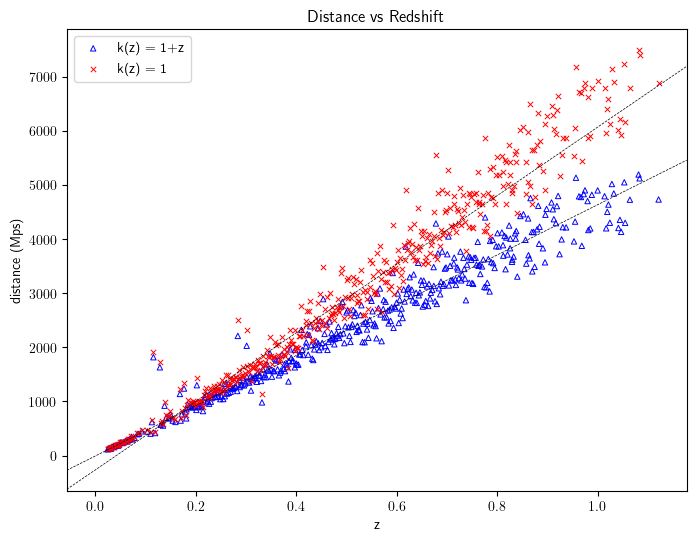
\includegraphics[width=\linewidth]{../graphs/mu_distance_vs_redshift.png}
  \caption{todo}
  \label{fig:corrected_uncalibrated}
\end{figure}

\begin{figure}[h!]
  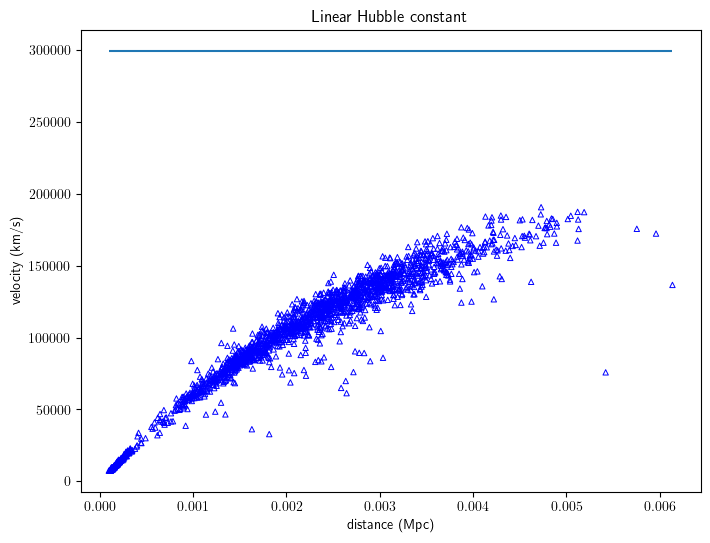
\includegraphics[width=\linewidth]{../graphs/velocity_vs_distance.png}
  \caption{todo}
  \label{fig:uncorrected_uncalibrated}
\end{figure}

\section{Calibrated distance models}
\label{sec:calibrated}

Calibrating a distance model involves finding a linear regression line for a
model and then computing the value $k$ required to make the regression model
match a Hubble paramater. By arbitrary choice, we use $H_0 = 70 \frac{km/s}{Mpsc}$.

The final units for distance will be in megaparsecs $Mpsc$. To find the
recessional speed for a given redshift, we use $v = cz$ where $c$ is the speed
of light.

To compute a model, we use non-parametric regression via repeated means as described in
\citet{siegel1982}. A comparison of both models is shown in Figure .


\section{Disagreement with existing research}

Previous studies use $F$ instead of $F*$. According to \citet{betoule2014},

\begin{equation}
  D_L = k 10^\frac{M}{5}.
\end{equation}

\section{Conclusions}
\label{sec:conclusions}

\bibliographystyle{unsrtnat}
\bibliography{references}

\end{document}
